\chapter{Convertitore Tensione-Frequenza}

%--------------------------------------------------------------------------------------------

Si vuole ora progettare il circuito per la generazione del segnale di clock, con le
specifiche ottenute dal capitolo precedente, ovvero:

\begin{itemize}
    \item Frequenza minima: $\approx 14kHz$;
    \item Frequenza massima: $\approx 3.6MHz$;
    \item Livello logico basso: $0V$;
    \item Livello logico alto: $+5V$;
\end{itemize}

%--------------------------------------------------------------------------------------------

\subsection*{Principio di Funzionamento}

%--------------------------------------------------------------------------------------------

Ciò di cui abbiamo bisogno è un circuito in grado di convertire una tensione in un segnale
a onda rettangolare con frequenza proporzionale alla tensione stessa, ovvero un convertitore
tensione-frequenza.

In commercio è possibile trovare diversi chip in grado di svolgere questa funzione
semplicemente aggiungendo una manciata di componenti di contorno, anche se la maggior
parte di questi non arriva a coprire l'intero range di funzionamento di cui abbiamo bisogno
(come ad esempio il noto LM331 \cite{lm331}). Nel nostro caso si utilizza un VFC110
\cite{vfc110}, circuito integrato che vanta un'ottima linearità e capace di fornire una
frequenza di $4MHz$ in uscita con una corrispondente tensione in ingresso di $10V$,
esattamente ciò che la nostra applicazione richiede.
\medskip

\begin{figure}[ht]
    \centering
    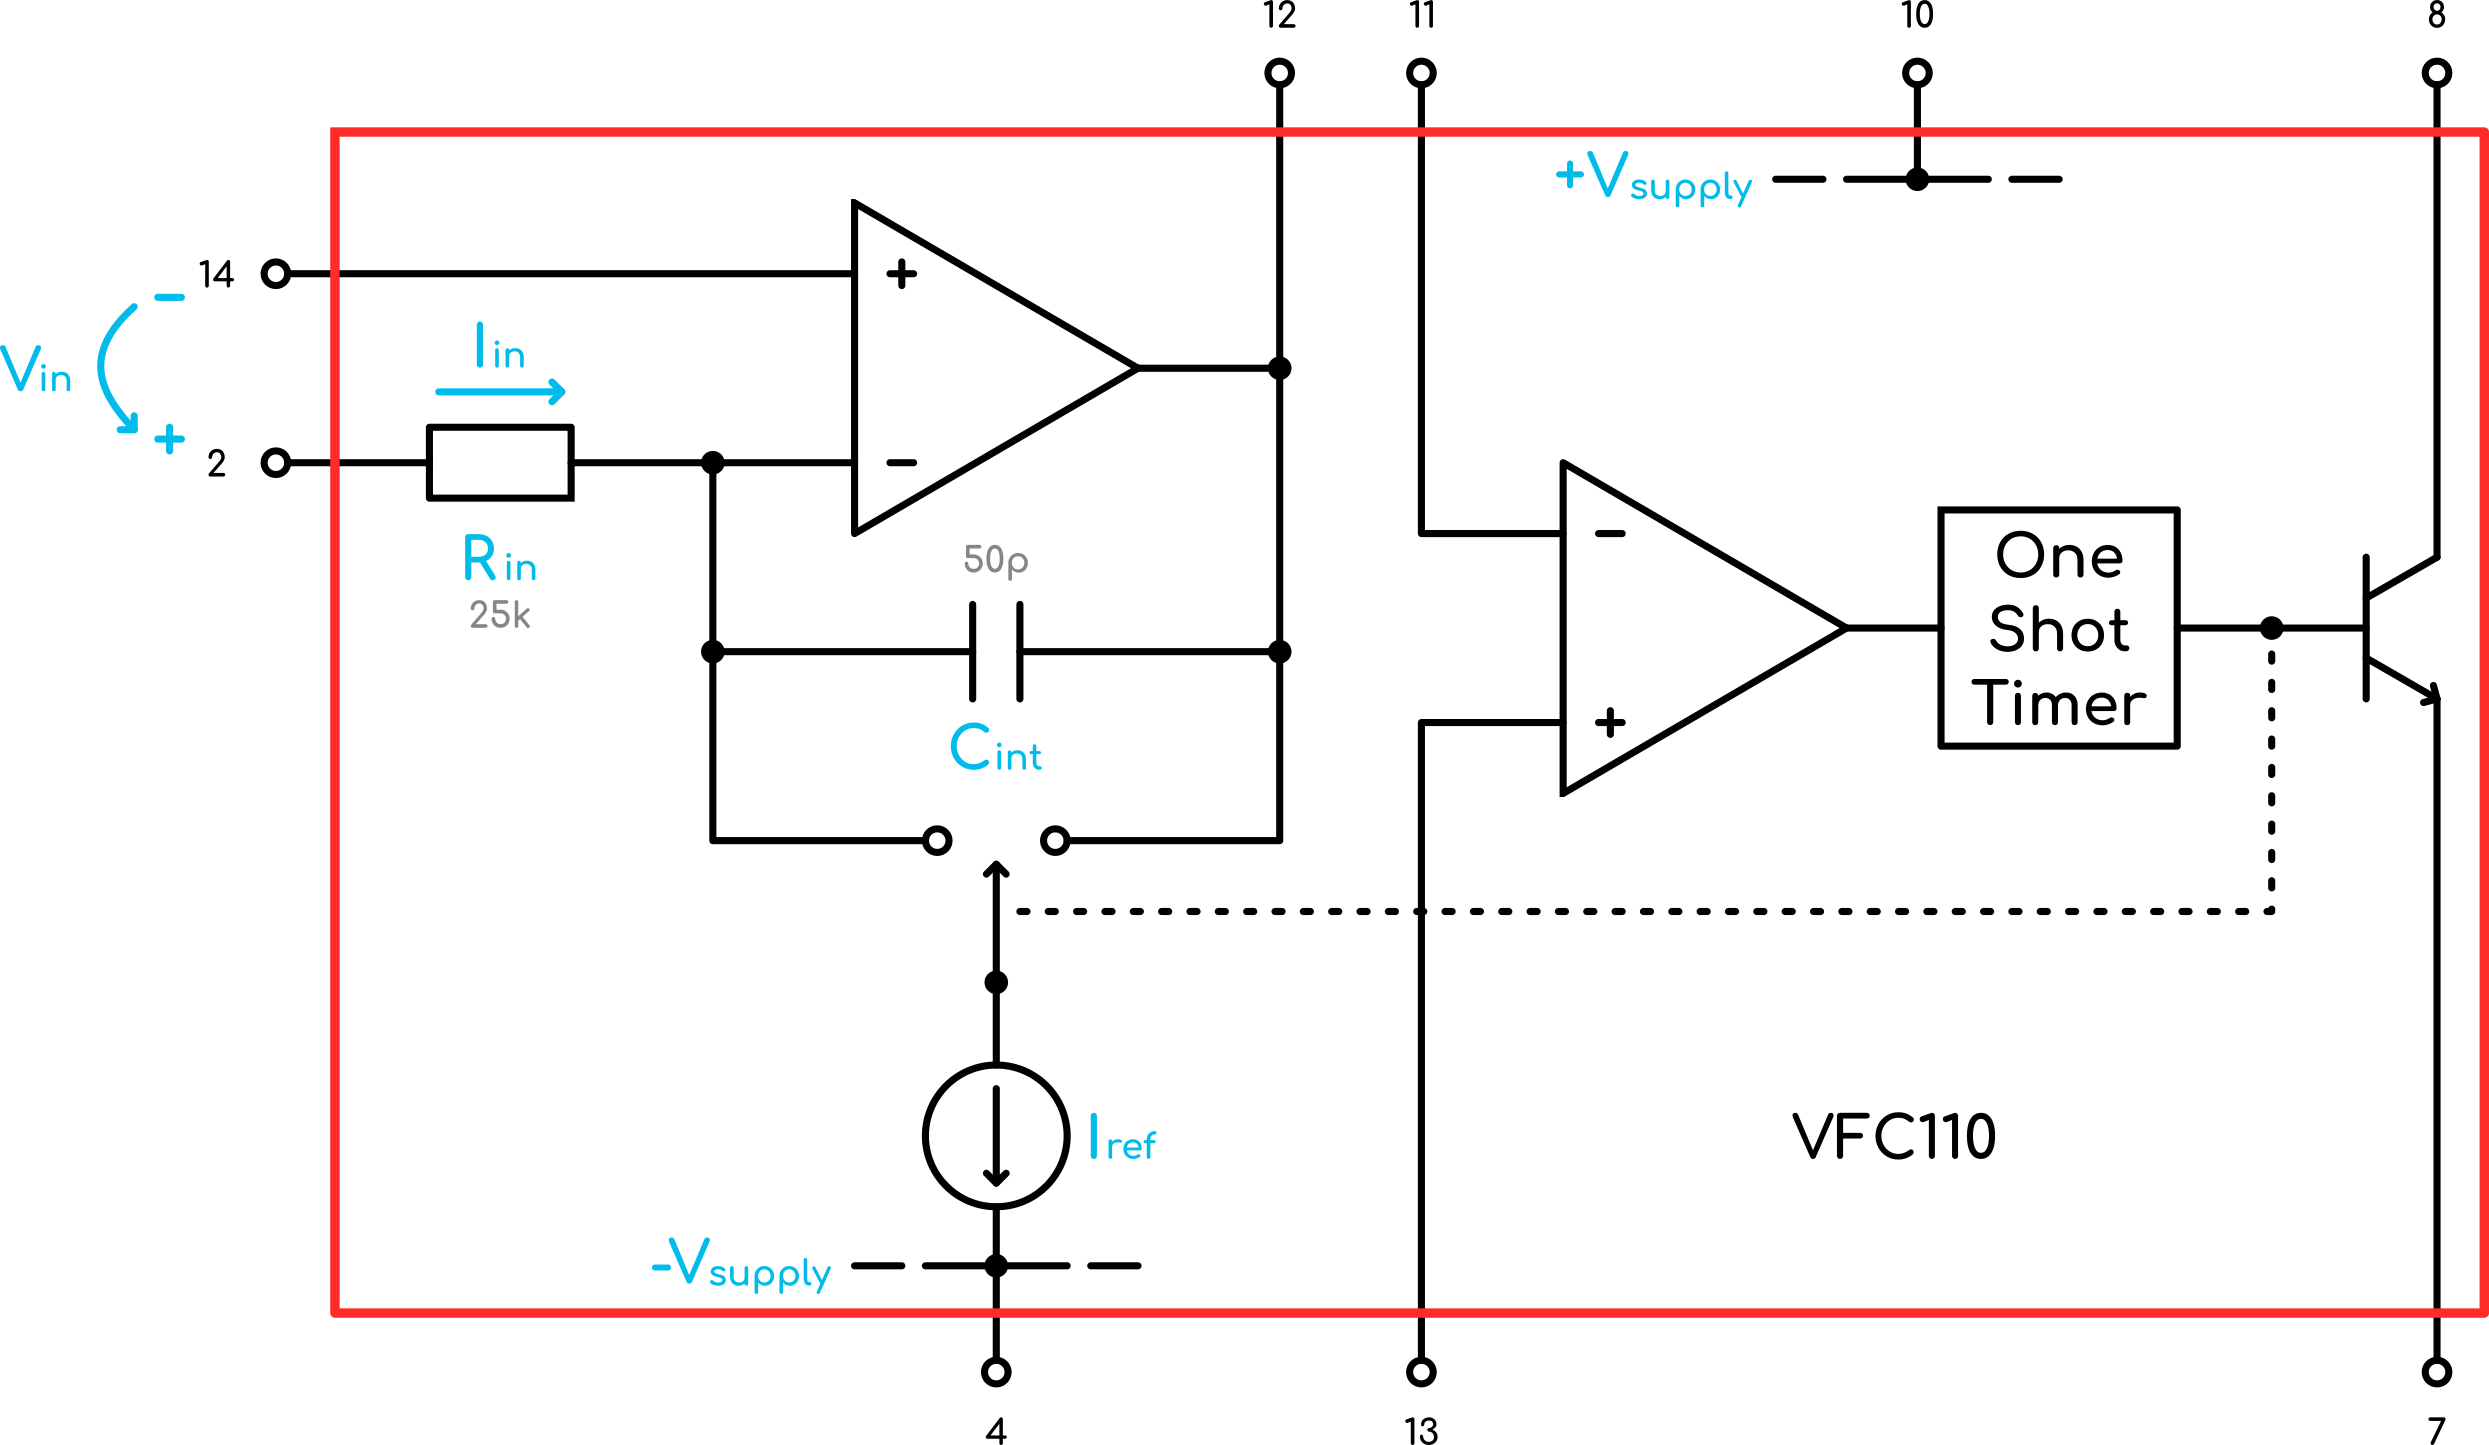
\includegraphics{circuits/vfc110_internal.png}
    \caption{Estratto della struttura interna di un VFC110}
    \label{vfc100_internal}
\end{figure}

Il cuore del circuito consiste in un operazionale configurato come integratore, con tensione
di uscita proporzionale alla carica immagazzinata nella sua capacità di feedback $C_{int}$.
Una tensione in ingresso $V_{in}$ sviluppa una corrente $I_{in}=\frac{V_{in}}{R_{in}}$
che viene forzata in $C_{int}$, causando quindi un andamento a rampa decrescente in uscita.
Arrivati a $0V$ il comparatore scatta, attivando il timer one-shot. Quindi un generatore
di corrente $I_{ref}$ (dal valore di circa $1mA$) viene connesso all'ingresso dell'integratore
per un periodo di durata pari a $T_{OS}$, causando un andamento a rampa crescente in uscita
all'integratore. Infine il ciclo ricomincia.

% immagine rampa e fout teoriche

Per uno studio più approfondito sul funzionamento del VFC110 si consiglia la lettura del
datasheet del componente, dal quale si ricava anche la configurazione del circuito utilizzato
per sfruttare l'intero range offerto. Si modificano però i valori di alimentazione con
quelli dello standard scelto ($\pm 12V$).
\medskip

\begin{figure}[ht]
    \centering
    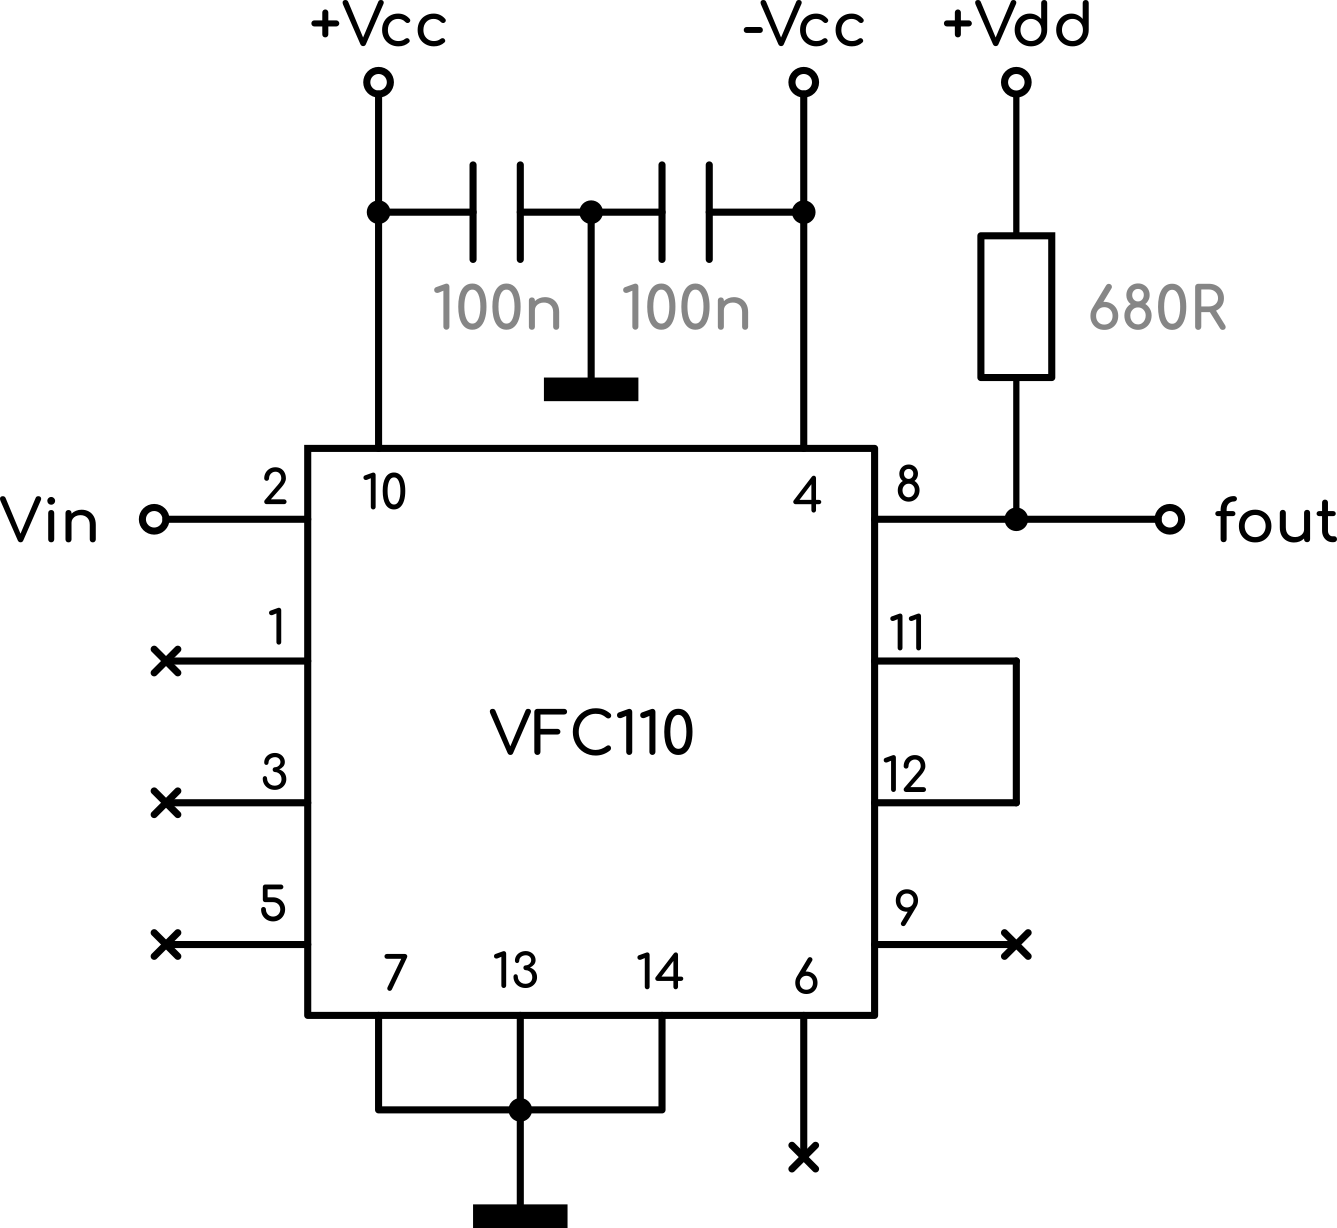
\includegraphics{circuits/VFC_circuit.png}
    \caption{Schema elettrico del VFC110 utilizzato}
    \label{VFC_circuit}
\end{figure}

Si noti che gli unici componenti aggiunti sono condensatori di filtro e un resistore di
pull-up per l'uscita a collettore aperto.

Le relazioni tra le grandezze in gioco sono le seguenti:

\begin{displaymath}
    I_{in}=I_{ref}\cdot\delta
    \qquad
    \rightarrow
    \qquad
    \delta=\frac{I_{in}}{I_{ref}}=\frac{V_{in}}{R_{in}\cdot I_{ref}}
\end{displaymath}

\begin{displaymath}
    \frac{V_{in}}{R_{in}}=I_{ref}\cdot f_{out}\cdot T_{OS}
    \qquad
    \rightarrow
    \qquad
    f_{out}=\frac{V_{in}}{R_{in}\cdot I_{ref}\cdot T_{OS}}=\frac{\delta}{T_{OS}}
\end{displaymath}

%--------------------------------------------------------------------------------------------

\subsection*{Risultati Pratici e Misure}

%--------------------------------------------------------------------------------------------

Si procede quindi alla verifica del corretto funzionamento del circuito. Il setup di
misura utilizzato viene riportato in figura:

% grafica setup di misura

Possiamo innanzitutto controllare il comportamento dell'integratore descritto al
paragrafo precedente:

\begin{figure}[ht]
    \centering

    \begin{subfigure}{.5\textwidth}
        \centering
        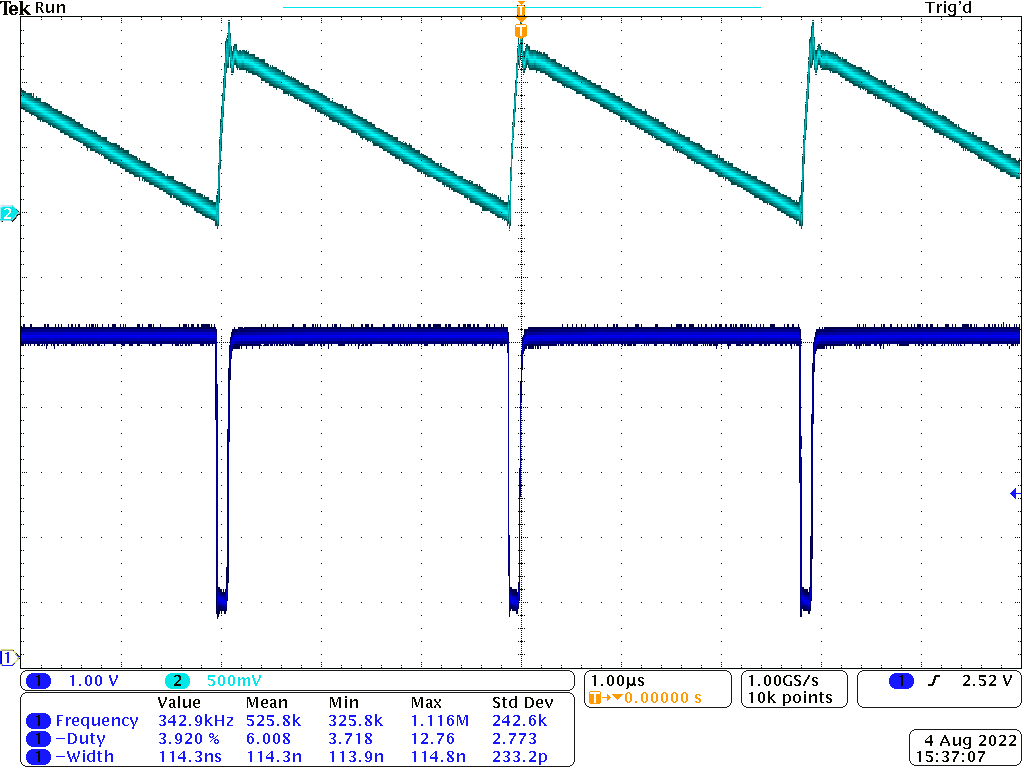
\includegraphics[scale = 0.2]{acquisitions/VFC_1V.png}
        \caption{$V_{in}=1V$}
        \label{acq_vfc110_1v}
    \end{subfigure}%
    \begin{subfigure}{.5\textwidth}
        \centering
        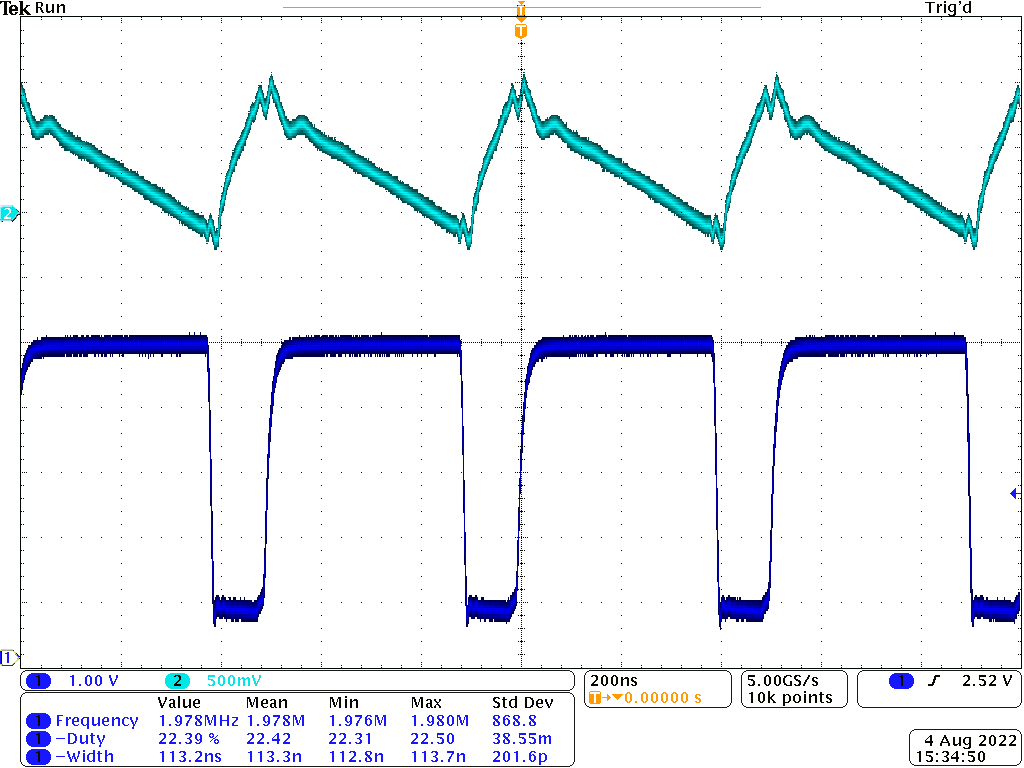
\includegraphics[scale = 0.2]{acquisitions/VFC_5V.png}
        \caption{$V_{in}=5V$}
        \label{acq_vfc110_5v}
    \end{subfigure}
    \begin{subfigure}{.5\textwidth}
        \centering
        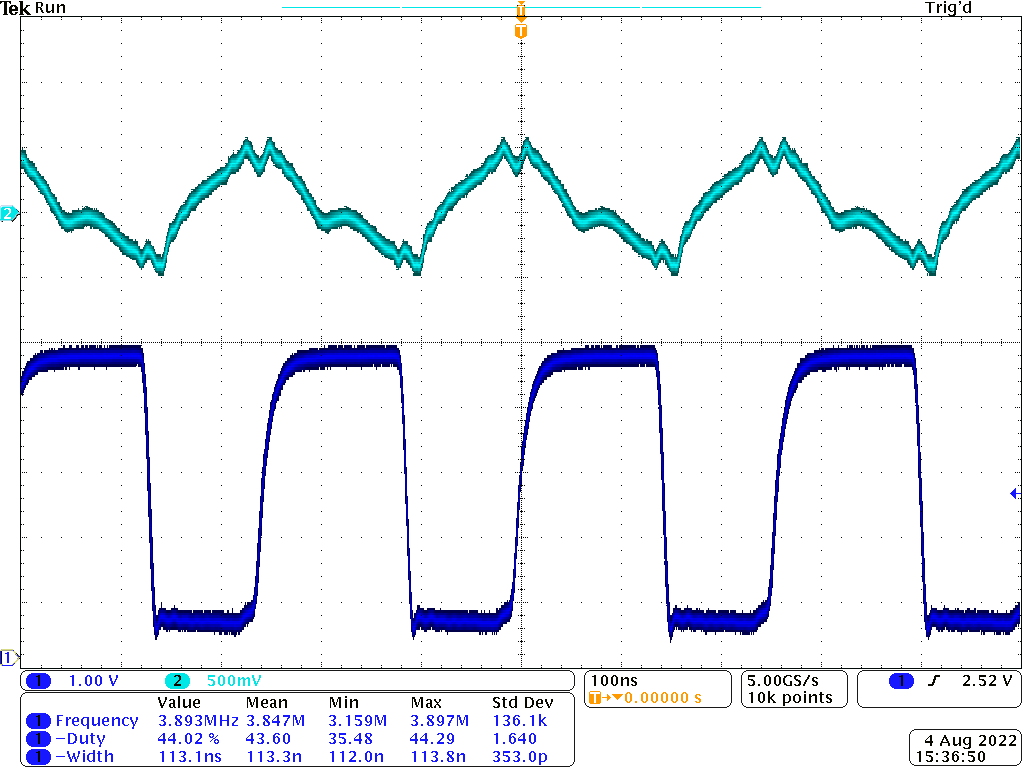
\includegraphics[scale = 0.2]{acquisitions/VFC_10V.png}
        \caption{$V_{in}=10V$}
        \label{acq_vfc110_10v}
    \end{subfigure}

    \caption{Acquisizioni dell'uscita dell'integratore (pin 12, ch.2) e $f_{out}$
        corrispondente (ch.1) per diversi valori di $V_{in}$}
    \label{acq_vfc110}
\end{figure}

Si nota che la durata del periodo basso di $f_{out}$ si setende lungo il tratto di rampa
crescente, come in figura.

Ora si raccolgono i dati per tracciare la transcaratteristica del circuito:

% tabella valori & transcaratteristica (grafico vin/duty/fout)
